\documentclass{article}

\usepackage[T1]{fontenc}
\usepackage[polish]{babel}
\usepackage[utf8]{inputenc}
\usepackage{amsmath}
\usepackage{hyperref}
\usepackage{tablefootnote}
\usepackage{graphicx}
\usepackage{siunitx}
\usepackage{listings}
\usepackage{xcolor}

\lstset{frame=tb,
  language=Python,
  aboveskip=3mm,
  belowskip=3mm,
  showstringspaces=false,
  columns=flexible,
  basicstyle={\small\ttfamily},
  numbers=none,
  numberstyle=\tiny\color{gray},
  keywordstyle=\color{blue},
  commentstyle=\color{dkgreen},
  stringstyle=\color{green},
  breaklines=true,
  breakatwhitespace=true,
  tabsize=3
}

\graphicspath{ {./media/} }

\begin{document}

\section{Cel ćwiczenia}
Celem cwiczenia jest pomiar oporu elektrycznego pojedynczych rezystorów
oraz układu rezystorów połaczonych szeregowo i równolegle z wykorzystaniem
mostka pradu stałego (mostek Wheatstone’a) wykorzystując przedstawiony na 
poniższym rysunku układ.

\begin{center}
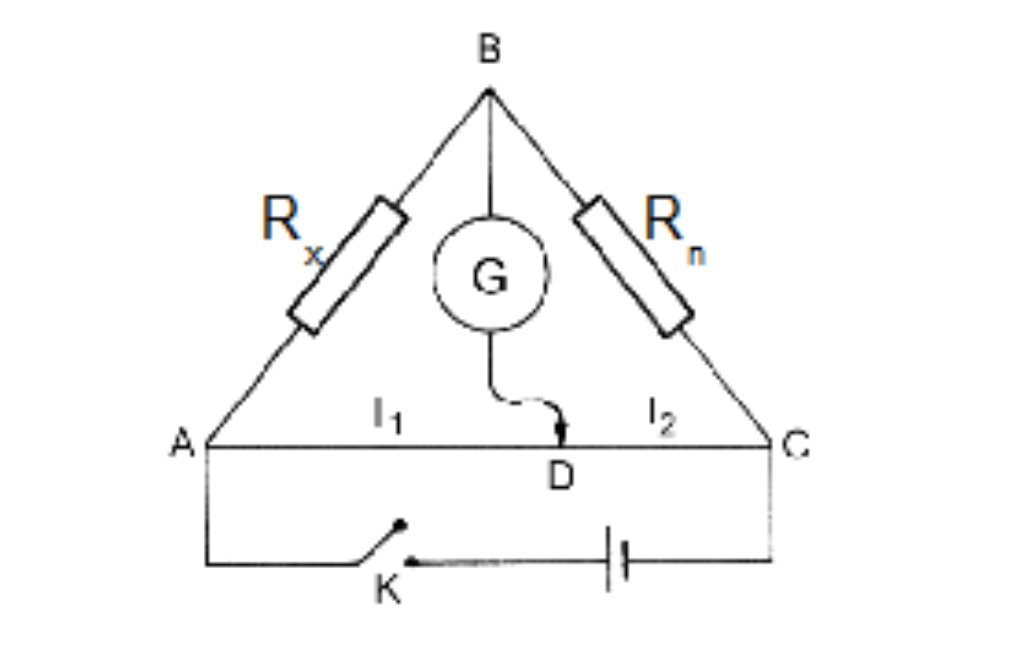
\includegraphics[width=10cm]{e3}
\end{center}
$R_n$ - rezystancja wzorcowa (rezystora dekadowego) \\
$R_x$ - badana rezystancja \\
$l_1, l_2$ - położenie ślizgacza na skali milimetrowej listy

\section{Użyte wzory}

\subsection{Wyniki}
Do obliczenia rezystancji $R_x$ przy wykorzystaniu pomierzonych danych korzystamy ze wzoru
\begin{gather*}
	R_x = R_n\frac{l_1}{l_2}
\end{gather*} 
Natomiast chcąc policzyć opór właściwy konstatanu korzystamy ze wzoru 
\begin{gather*}
	R(\frac{1}{d^2}) = \frac{\rho * l}{\pi} * \frac{1}{d^2}
\end{gather*}
stąd współczynnik kierunkowy prostej otrzymanej z metody najmniejszych kwadratów będzie równy
\begin{gather*}
	a = \frac{\rho * l}{\pi} 
\end{gather*}
\subsection{Niepewności}
Ponieważ opornik dekadowy jest bardzo dokładny, w dalszych rozważaniach uznajemy, że jego niepewność jest równa zeru.
Niepewność rezystancji liczyliśmy zatem z metody różniczki zupełnej uwzględniając niepewności $l_1$ i $l_2$ \footnote{\url{https://ftims.pg.edu.pl/documents/10673/20436990/wstep.pdf} (9.)}
\begin{gather*}
	\Delta R_x = |\frac{\partial R_x}{\partial l_1}|\Delta l_1+ |\frac{\partial R_x}{\partial l_2}|\Delta l_2 = \frac{R_n}{l_2}(\Delta l_1 + \frac{l_1}{l_2} \Delta l_2) \\
	\Delta R_x = R_x (\delta l_1+ \delta l_2)
\end{gather*}
przyjmując $\Delta l_i = 1$mm. \\
Do określenia niepewności oporu właściwego konstatanu skorzystamy ze wzoru \footnote{\url{https://ftims.pg.edu.pl/documents/10673/20436990/wstep.pdf}}\\
\begin{gather*}
		u_a = \sqrt{\frac{n}{n-2} * \frac{\Sigma y_i^2 - a\Sigma x_iy_i}{n\Sigma x_i^2}} 
\end{gather*}
skąd
\begin{gather*}
		u_\rho = |\frac{\partial \rho}{\partial a}| u_a = \frac{\pi}{l}u_a
\end{gather*}

\section{Badanie rezystancji pojedynczych rezystorów o nieznanej wartości}
\subsection{Pomierzone dane}
\begin{center}
\begin{tabular}{ c | c | c | c}
Rezystor & $R_n$ [\si{\ohm}] & $l_1$ [mm] & $l_2$ [mm]\\
\hline
 1    & 152 & 480 & 520\\ 
 2    & 620 & 506 & 494\\ 
 3  & 430 & 504 & 496\\ 
 4  & 2040 & 501 & 499\\
 5   & 3030 & 502 & 498\\
 6  & 13800 & 500 & 500\\
 
\end{tabular}
\end{center}

\subsection{Wyniki}
\begin{center}
\begin{tabular}{ c | c }
Rezystor & $R_x$ [\si{\ohm}]\\
\hline
 1    & 140,31 $ \pm$  0,56\\ 
 2    & 635,06 $\pm$ 2,53\\ 
 3  & 437,94 $\pm$ 1,75\\ 
 4  & 2048,18 $\pm$ 8,19\\
 5   & 3054, 34 $\pm$ 12,22\\
 6  & 13800,00 $\pm$ 55,20\\

\end{tabular}
\end{center}

\subsection{Rachunek niepewności}



\section{Badanie rezystancji układów rezystorów połączonych szeregowo}
\subsection{Pomierzone dane}
\begin{center}
\begin{tabular}{ c |  c | c | c}
Rezystor & $R_n$ [\si{\ohm}] & $l_1$ [mm] & $l_2$ [mm]\\
\hline 
 4 i 2 & 2720 & 500 & 500\\ 
 5 i 2 & 3780 & 500 & 500\\ 
4 i 5 & 5000 & 508 & 492\\ 
\end{tabular}
\end{center}

\subsection{Wyniki}
\begin{center}
\begin{tabular}{ c | c }
Rezystor & $R_x$ [\si{\ohm}]\\
\hline
 2 i 4  & 2720,00 $\pm$ 10,88\\ 
 2 i 5  & 3780, 00 $\pm$ 15,12\\ 
 4 i 5  & 5163,60 $\pm$ 20,66\\ 
\end{tabular}
\end{center}
\section{Badanie rezystancji układów rezystorów połączonych równolegle}
\subsection{Pomierzone dane}
\begin{center}
\begin{tabular}{ c |  c | c | c}
Rezystor & $R_n$ [\si{\ohm}] & $l_1$ [mm] & $l_2$ [mm]\\
\hline
 2 i 4 & 495 & 500 & 500\\ 
 2 i 5 & 540 & 500 & 500\\ 
 4 i 5 & 1260 & 499 & 501\\ 
\end{tabular}
\end{center}


\subsection{Wyniki}
\begin{center}
\begin{tabular}{ c | c }
Rezystor & $R_x$ [\si{\ohm}]\\
\hline
2 i 4    & 495,00 $\pm$ 1,98\\ 
2 i 5  & 540,00 $\pm$ 2,16\\ 
4 i 5    & 1254,97 $\pm$ 5,02\\ 

\end{tabular}
\end{center}

\section{Badanie drutów konstantanowych o różnej średnicy}
\subsection{Pomierzone dane}

\begin{center}
\begin{tabular}{ c |  c | c | c}
d [mm] & $R_n$ [\si{\ohm}] & $l_1$ [mm] & $l_2$ [mm]\\
\hline
 0,35 & 5 & 503 & 497\\ 
 0,50 & 2 & 544 & 456\\ 
 0,70 & 1 & 547 & 453\\ 
 1,00 & 1 & 365 & 635\\ 

\end{tabular}
\end{center}
{d} - średnica drutu\\
$R_n$ - opór wzorcowy mostka\\ 
$l_1$ - położenie ślizgacza na skali milimetrowej listwy\\

\subsection{Wyniki}
\begin{center}
\begin{tabular}{ c|c | c }
$d$ [mm] & $\frac{1}{d^2}$ [mm$^{-2}]$ &$R_x$ [\si{\ohm}]\\
\hline
0,35 & 8,16 & 5,06$\pm$ 0,02\\ 
 0,50 & 4,00 &2,39 $\pm$ 0,01\\ 
 0,70 & 2,04 &1,21 $\pm$ 0,01\\ 
 1,00 & 1,00 &0,57 $\pm$ 0,01\\ 
 
\end{tabular}
\end{center}

\subsection {Zależność R =$ f(\frac{1}{d^2})$}
\begin{center}
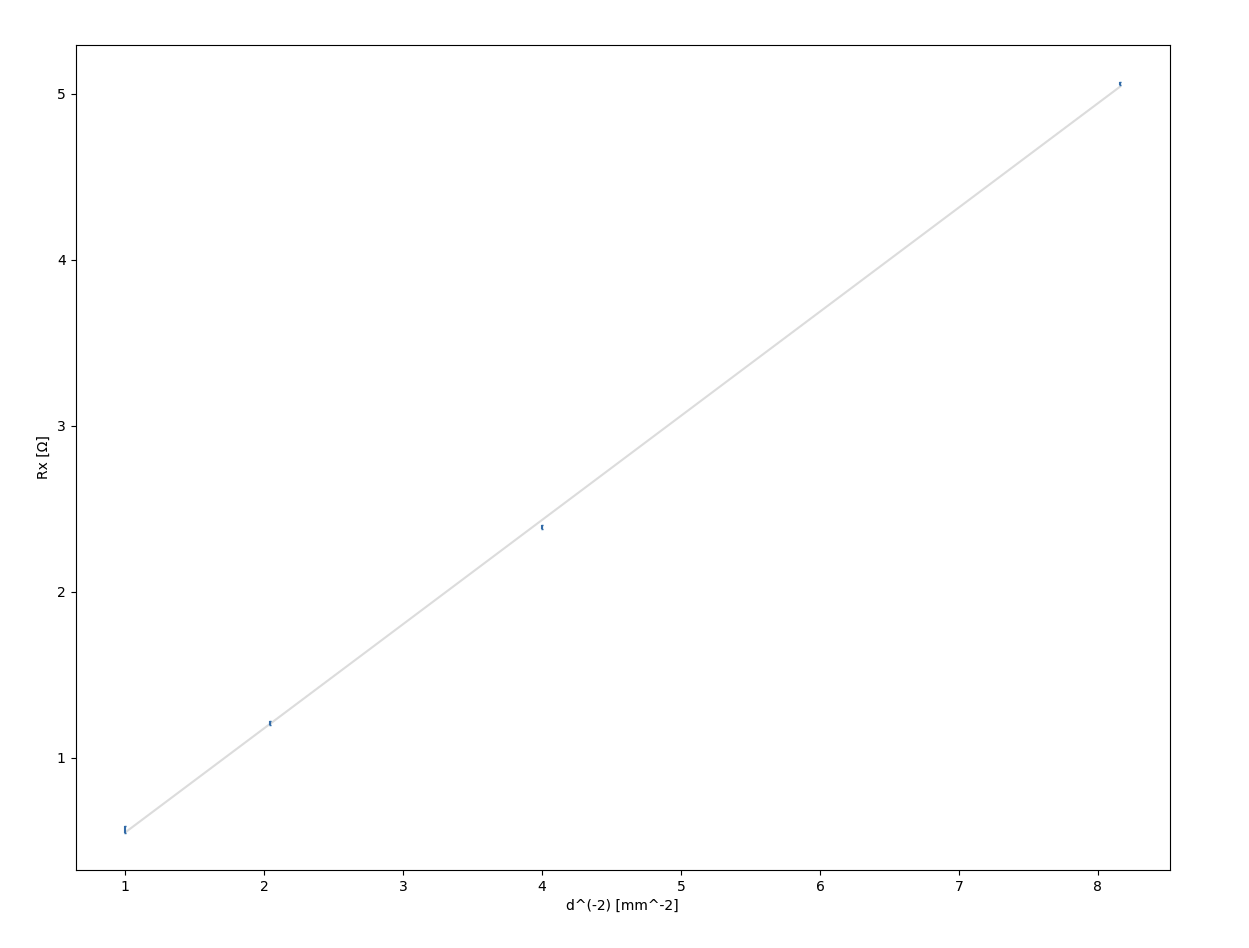
\includegraphics[width=15cm]{e3_wykres}
\end{center}
a = 0,63 $\rightarrow$ $\rho$ = (1,88  $\pm$ 1,97 ) * 10$^{-6} \Omega$m (korzystamy z wzorów wymienionych wyżej)
niech ktoś to jeszcze przeliczy czy się nie zajebałem w jednostkach (w pythonie to jest ta funkcja stdev)

\subsection{Kod w pythonie}
Kod użyty do narysowania wykresu i policzenia $u_\rho$
\begin{lstlisting}[language=Python]
import math

import matplotlib
import matplotlib.pyplot as plt
import numpy as np

from matplotlib.pyplot import plot, show, errorbar, savefig


def stdev(a, x, y): 
    n = len(y)
    numerator = abs(sum([i * i for i in y]) - a * sum([x[i]*y[i] for i in range(n)]))
    denominator = n * sum([i * i for i in x])

    return math.sqrt(n/(n-2) * numerator / denominator)


if __name__ == "__main__":
    matplotlib.use('MacOSX')

    error = [0.02, 0.01, 0.01, 0.01]
    x = [1.0, 2.04, 4.0, 8.16]
    y = [0.57, 1.21, 2.39, 5.06]

    coeff = np.polyfit(x,y,1)
    dev = stdev(coeff[0], x, y)

    plot(x,y, 'yo', x, np.poly1d(coeff)(x),  c='0.88',markersize=0.01)
    _, caps, _ = errorbar(x, y, error, fmt='o',  markersize=0.01, capsize=1)

    for cap in caps:
        cap.set_markeredgewidth(1)

    plt.ylabel('Rx [\Ohm]')
    plt.xlabel('d^(-2) [mm^-2]')

    print("a=", coeff)
    print("stdev=", dev)

    show()

\end{lstlisting}


\section{Wnioski}

Wyniki pomiarów były dokładniejsze ze względu na poprawne równoważenie mostka w centralnej części struny \\

Wyniki pomiarów rezystancji szeregowo i równolegle zgadzają się z wartościami teoretycznymi\\

Szeregowo:

\begin{center}
    \begin{tabular}{ c | c | c }
    Rezystor & $R_x$ [\si{\ohm}] & Wartość teoretyczna [\si{\ohm}]\\
    \hline
     2 i 4  & 2720,00 $\pm$ 10,88& 2683,24\\ 
     2 i 5  & 3780, 00 $\pm$ 15,12 & 3689,40\\ 
     4 i 5  & 5163,60 $\pm$ 20,66&  5103,51\\ 
    \end{tabular}
\end{center}

Równolegle:

\begin{center}
    \begin{tabular}{ c | c | c}
    Rezystor & $R_x$ [\si{\ohm}] & Wartość teoretyczna [\si{\ohm}]\\
    \hline
    2 i 4    & 495,00 $\pm$ 1,98 & 485,76\\ 
    2 i 5  & 540,00 $\pm$ 2,16 & 525,75\\ 
    4 i 5    & 1254,97 $\pm$ 5,02 &  1226,03\\ 
    
    \end{tabular}
\end{center}

Wyniki pomiarów rezystancji drutów są zbliżone do wartości teoretycznych. Różnice między wartościami mogły być spowodowane niedokładnością pomiaru długości drutu oraz nie wzięciem pod uwagi temperatury.\\\\
Opór właściwy konstantanu wynosi $\rho$ = $0.5*10^{-6} \si{\ohm}m$

\begin{center}
    \begin{tabular}{ c|c | c|c }
    $d$ [mm] & $\frac{1}{d^2}$ [mm$^{-2}]$ &$R_x$ [\si{\ohm}] & Wartość teoretyczna [\si{\ohm}]\\
    \hline
    0,35 & 8,16 & 5,06$\pm$ 0,02 & 4,08\\ 
     0,50 & 4,00 &2,39 $\pm$ 0,01 & 2,00\\ 
     0,70 & 2,04 &1,21 $\pm$ 0,01 & 1,02\\ 
     1,00 & 1,00 &0,57 $\pm$ 0,01 & 0,50\\ 
     
    \end{tabular}
\end{center}

\end{document}